\documentclass{tufte-handout}

%\geometry{showframe}% for debugging purposes -- displays the margins

\usepackage{amsmath}

% Set up the images/graphics package
\usepackage{graphicx}
\setkeys{Gin}{width=\linewidth,totalheight=\textheight,keepaspectratio}
\graphicspath{{graphics/}}

\title{TCA Cycle and the Electron Transport Chain}
\author{}
\date{}  % if the \date{} command is left out, the current date will be used

% The following package makes prettier tables.  We're all about the bling!
\usepackage{booktabs}

% The units package provides nice, non-stacked fractions and better spacing
% for units.
\usepackage{units}

% The fancyvrb package lets us customize the formatting of verbatim
% environments.  We use a slightly smaller font.
\usepackage{fancyvrb}
\fvset{fontsize=\normalsize}

% Small sections of multiple columns
\usepackage{multicol}

% Provides paragraphs of dummy text
\usepackage{lipsum}

% These commands are used to pretty-print LaTeX commands
\newcommand{\doccmd}[1]{\texttt{\textbackslash#1}}% command name -- adds backslash automatically
\newcommand{\docopt}[1]{\ensuremath{\langle}\textrm{\textit{#1}}\ensuremath{\rangle}}% optional command argument
\newcommand{\docarg}[1]{\textrm{\textit{#1}}}% (required) command argument
\newenvironment{docspec}{\begin{quote}\noindent}{\end{quote}}% command specification environment
\newcommand{\docenv}[1]{\textsf{#1}}% environment name
\newcommand{\docpkg}[1]{\texttt{#1}}% package name
\newcommand{\doccls}[1]{\texttt{#1}}% document class name
\newcommand{\docclsopt}[1]{\texttt{#1}}% document class option name

\begin{document}

\maketitle% this prints the handout title, author, and date

\begin{abstract}
\noindent The aquisition and utilization of mitochondria during evolution dramatically improved the ability of the cell to generate energy.  In the presence of oxygen and ATP demand, the products of glycolysis, amino acid catabolism and lipid oxidation enter the TCA Cycle\sidenote{Also known as the Tricarboxylic Acid Cycle, Kreb's Cycle or Citric Acid Cycle.}.  This allows for complete oxidation of metabolites into CO\textsubscript{2} and efficient energy production by the mitochondrial ATP synthase.  This unit will describe how the TCA Cycle and Electron Transport Chain are regulated, and how various nutrients interact with this cellular pathway.  For more details about the these topics see Chapters 18-20 in Biochemistry: A Short Course\cite{Berg2015}, available on reserve.
\end{abstract}
%add chapters
\tableofcontents
\pagebreak
\section{Learning Objectives}

\begin{itemize}
\item Evaluate the potential metabolic fates of pyruvate and the signals that control these changes.
\item Assess the importance of the mitochondria in glucose metabolism.
\item Describe the key regulatory nodes of the TCA cycle.
\item Understand the concepts of anaplerosis and cataplerosis and how this can affect TCA cycle efficiency.  Predict whether a particular pathway is anaplerotic or cataplerotic.
\item Explain the differences in efficiency between anaerobic glycolysis and the TCA cycle linked to the electron transport chain.
\item Recall the key functions of the electron carriers NADH, FADH\textsubscript{2} and QH\textsubscript{2}.
\item Calculate ATP production from GTP, NADH and FADH\textsubscript{2} equivalents.
\item Understand how mitochondria balance nutrient flux with ATP requirements.
\end{itemize}

\section{Key Vocabulary and Concepts}
\begin{itemize}
	\item Anaplerosis
	\item Cataplerosis
	\item Electron Carrier Molecules (including NADH, FADH\textsubscript{2} and QH\textsubscript{2})
	\item Proton Gradients and the Electromotive Force
	\item Oxidative Stress, Antioxidants, and Reactive Oxygen Species
\end{itemize}

\section{The Next Steps in Carbohydrate Metabolism Require Mitochondria}
While glucose oxidation to the level of Pyruvate generates the equivalent of 7 ATP molecules\sidenote{2 x NADH (5 ATP equivalents at 2.5 ATP/NADH) and 2 x ATP are generated.}, full oxidation to CO$_2$ can yield up to 32 molecules of ATP.  This process requires transport of pyruvate into the mitochondria where Acetyl-CoA is generated and degraded to CO$_2$, GTP and reduction of electron carrier molecules.  These molecules, NADH and FADH\textsubscript{2} are passed to the electron transport chain, generating a proton gradient, which powers the mitochondrial ATPase\sidenote{This is a little confusingly named, as an "ase" generally can break down a molecule.  In this case the mitochondrial ATPase \emph{generates} ATP from ADP.}.  Mitochondria are also the only way to catabolize fatty acids, and most Amino Acids.  As a membrane-enclosed organelle, many key metabolites are impermeable to mitochondria without transporters.  These include cytoplasmic NADH generated during glycolysis as well as Pyruvate.  Fortunately there are a variety of transporters and shuttle systems that transport key materiel from the cytoplasm into the mitochondria \sidenote{For more details see \url{https://www.ncbi.nlm.nih.gov/books/NBK22470/}.}.

\subsection{Regulation of Mitochondrial Numbers}
Before we start with what happens in mitochondria, its worth taking a step back and considering how mitochondrial amounts are regulated.  The presence of mitochondria is essential for aerobic metabolism, and muscle fibers that are rich in mitochondria are able to fully oxidize glucose and other fuels.  These are known as Type I muscle fibers, or colloquially as slow-twitch muscle fibers\sidenote{There is another fast-twitch fiber type that contains less mitochondria called IIA fibers}.  The number and efficiency of mitochondria in muscle is not static, and can be modified by training.  For example endurance training dramatically increases the number of mitochondria and the levels of TCA and ETC enzymes in both rodent and human studies \citep{Holloszy1967,Gollnick1972,Gollnick1973}.  Understanding the molecular mechanisms by which this happens is a major research area both in terms of human performance, and in terms of modifying energy expenditure and promoting healthy aging (for more details see \citet{Cartee2016}).  Some cells have few or no mitochondria.  In this case they are entirely dependent on glycolysis for ATP production.

\section{The Possible Fates of Pyruvate}

As we discussed in the unit on glycolysis, pyruvate has several possible fates.  If Alanine levels are low and Glutamate levels are high, Pyruvate can be converted to Alanine via ALT\sidenote{Alanine Aminotransferase.}.  If there is energy demand, PDH\sidenote{Pyruvate Dehdyrogenase, discussed in the next section.} is activated and pyruvte becomes Acetyl-CoA.  If Acetyl-CoA levels are high, Pyruvate becomes the TCA Cycle intermediate Oxaloacetate via the actions of Pyruvate Carboxylase.  If none of these enzymes are activated, Pyruvate is converted by Lactate Dehydrogenase and released from the cell as Lactate.  The reversible Lactate Dehydrogenase reaction is:

\begin{equation}\label{eq:ldh}
Pyruvate + NADH \rightleftharpoons Lactate + NAD^+
\end{equation}

\subsection{Anaerobic Glycolysis}
If oxygen is unavailable to the cell, or there are no mitochondria present and lactate is produced, this is the end of anaerobic glycolysis.  The reaction to generate lactate uses up the NADH produced during glycolysis.  This means that on net one glucose molecule now generates just two ATP equivalents\sidenote{Walk yourself through this to convince yourself this is correct.}.  The lactate molecule that is released was once thought to be primarily converted back to glucose by a pathway called the Cori cycle\sidenote{This will be explained in more detail when we discuss gluconeogenesis.} but recent experiments monitoring the flux of lactate shows that a large fraction of lactate is anaplerotic, meaning it is used to increase the number of molecules in the TCA cycle \citep{Hui2017,Ferguson2018}\sidenote{Anaplerosis and its inverse, cataplerosis will be described below.  If you are interested in understanding metabolic flux or the details of this study, there is a group bonus assignment about it on GradeCraft called Research Reflections - Lactate Flux and the use of Stable Isotopes.}.

\begin{margintable}
\centering
\caption{Potential fates of Pyruvate.}
\label{tab:pyruvate-fates}
\begin{tabular}{ccc}
\hline
\textbf {Pyruvate Fate} & \textbf{Conditions}  & \textbf{Key Enzyme} \\
\hline
TCA cycle & High PDH Activity & PDH \\
Lactate & Low PDH Activity & PDH \\
Alanine & Low Ala, High Glu & ALT\\
Oxaloacetate & High Acetyl-CoA & PC \\
\hline
\end{tabular}
\end{margintable}


\subsection{Regulation of Pyruvate Dehydrogenase}

Pyruvate Dehydrogenase\sidenote{This enzyme uses multiple cofactors, including Vitamin B1-derived TPP, Vitamin B2-derived FAD, vitamin B3-derived NAD and Vitamin B5-derived Coenzyme A.  Reduced PDH activity is a major cause of Beriberi and Wernicke-Korsakoff syndrome ( which are deficiencies of Vitamin B1.} is a mitochondrial enzyme that catalyzes this irreversible reaction:

\begin{equation}
Pyruvate + NAD^+ + CoA \rightarrow AcetylCoA + CO_2 + NADH +H^+
\end{equation}

The two most important products here are Acetyl-CoA, which will enter the TCA cycle and NADH which will go to Complex I of the Electron Transport Chain.  As one of the most important molecular decision steps, it makes sense that this enzyme is tightly regulated.  Intracellularly, PDH activity is turned on when energy is low, and turned off when energy is available.  The specific regulators are shown in Table \ref{tab:pdh-regulators} and Figure \ref{fig:pdh-pdk}.  The first several of these should be familiar to you, as increased substrate, and decreased energy (as sensed by low ATP, high ADP and low NADH, Acetyl-CoA) all promote PDH activity\sidenote{Now you may be thinking, I thought the key determinant of aerobic respiration was oxygen availability!  It may not be clear yet, but once you have read these notes, try to come back to this and think about how low oxygen levels would result in changes in PDH activity}.  Ca\textsuperscript{2+} is an activator of PDH activity, and as we will describe, also plays a role in activating several other TCA Cycle enzymes.  This is because, when muscles contract they release Calcium.  This allows for mitochondria to respond to contraction by generating more ATP.

\begin{marginfigure}
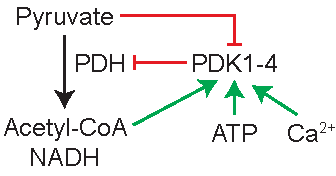
\includegraphics{figures/pdk-regulation.pdf}
\caption{Regulation of pyruvate dehydrogenase.}
\label{fig:pdh-pdk}
\end{marginfigure}

\newthought{Much like PFK2 and Pyruvate Kinase, PDH is Inhibited by Protein Phosphorylation.}  The phosphorylation of PDH is regulated by a specific protein kinase (PDH Kinase or PDK) which adds a phosphate group to PDH and reduces its activity (see Figure \ref{fig:pdh-pdk}).  The overall mechanism of regulation of PDH therefore is a combination of direct inhibitors of PDH (NADH and Acetyl-CoA), activators of the inhibitory kinase (ATP, Acetyl-CoA, NADH) and activators of the activating phosphatase (Ca\textsuperscript{2+}).  Unlike PFK1 and Pyruvate Kinase, PDK activity is regulated mostly at the metabolite level and not acutely by hormonal signals. 

\newthought{Pyruvate Dehydrogenase Kinase is regulated transcriptionally.}  While the activity of PDK is primarily regulated by metabolites, the number of PDK enzymes can be induced by several signals.  Here are a couple, as you read these take a moment to think \emph{why} this stimuli would alter PDK levels, and what would be the effects on glycolysis, gluconeogenesis and mitochondrial respiration.  Remember more PDK means \emph{less} PDH activity:

\begin{itemize}
	\item Glucocorticoids induce PDK4 transcription via FOXO \citep{Connaughton2010a}.
	\item Starvation induces PDK4 \citep{WU1998}.
	\item Insulin reduces PDK4 levels, insulin resistance elevates PDK4 levels \citep{Harris2001}.
	\item Hypoxia (low oxygen) induces PDK1 via HIF1$\alpha$ \citep{Kim2006}.
\end{itemize}

\begin{margintable}
\centering
\caption{Regulators of Pyruvate Dehydrogenase.}
\label{tab:pdh-regulators}
\begin{tabular}{ccc}
\hline
\textbf {Regulator} & \textbf{Effect} &\textbf{Mechanism}  \\
\hline
Pyruvate & Positive & Inactivates PDK\\
ADP & Positive & Inactivates PDK\\
ATP & Negative & Activates PDK\\
Acetyl-CoA & Negative &  Activates PDK, Inhibits PDH\\
NADH & Negative & Inhibits PDH\\
Ca\textsuperscript{2+} &  Positive & Activates PDH Phosphatase \\
\hline
\end{tabular}
\end{margintable}

\newthought{Acetyl-CoA also enters the TCA Cycle after $\beta$-oxidation.}  While we have focused so far on carbohydrate metabolism, now is a good time to talk briefly about lipid oxidation.  Unlike carbohydrates, when fatty acids are broken down they produce Acetyl-CoA, not Pyruvate\sidenote{They also generate equal amounts of NADH, FADH\textsubscript{2} which we will discuss later}.  This means that in humans, fatty acids enter the TCA cycle here.  If fatty acids are oxidized in the liver, but the TCA Cycle is not activated, those extra Acetyl-CoA molecules are released as ketone bodies, which can be used by other tissues, after re-conversion back into Acetyl-CoA.

\newthought{Some amino acids are also converted into Acetyl-CoA.}  As we will learn in the gluconeogenesis and amino acid catabolism lectures, some amino acids, depending on the circumstances are able to become converted into glucose\sidenote{These are the glucogenic amino acids.}.  Others are converted into Acetyl-CoA and are known as the ketogenic amino acids.  These amino acids can only be oxidized into energy by entering the TCA cycle as Acetyl-CoA, but cannot become glucose\sidenote{Later we will learn that the exclusively ketogenic amino acids are Leucine and Lysine.  Phenylalanine, Isoleucine, Threonine, Tryptophan and Tyrosine are partially glucogenic and partially ketogenic.}.

\section{The TCA Cycle Products}

The TCA Cycle/ETC completely oxidizes Acetyl-CoA to CO\textsubscript{2}.  One cycle, using one molecule of Acetyl-CoA generates the following:

\begin{table}
\centering
\caption{TCA Cycle ATP generation.  See Table \ref{tab:atp-equivalents} for details on conversion rates.}
\label{tab:atp-tca}
\begin{tabular}{ccc}
\hline
\textbf {Product} & $\rightarrow$ & \textbf{ATP}\\
\hline
3 NADH & $\rightarrow$ & 7.5 ATP \\
1 FADH\textsubscript{2} & $\rightarrow$ &  1.5 ATP  \\
1 GTP & $\rightarrow$ &  1 ATP  \\
\hline
Total & & \textbf{10 ATP}\\
\end{tabular}
\end{table}

if we include the NADH generated by Pyruvate Dehydrogenase, that means that Pyruvate oxidation results in 12.5 molecules of ATP.  Based on what we have discussed in this unit and in the glycolysis unit, try to determine how much ATP is generated from one molecule of glucose\sidenote{For a slightly bigger challenge, consider that palmitate oxidation generates 8 Acetyl-CoA, 7 NADH and 7 FADH\textsubscript{2} molecules, but requires 2 ATP molecules for activation.  Consider the energy yield from a C16:0 (Palmitate) fatty acid, compared to glucose.}.  Compare this to the two molecules of ATP generated by anaerobic glycolysis and it should make sense why we breathe heavier when we exercise.

\subsection{NADH and FADH\textsubscript{2} Are Substrates for the Electron Transport Chain}
Once Acetyl-CoA is generated by PDH, or by the breadown of amino or fatty acids, the TCA cycle functions to extract electrons from these substrates and pass them along to the electron transport chain.  This is done by transferring electrons from TCA intermediates to electron carrier molecules including NADH and FADH\textsubscript{2}.  These molecules are "charged" by these electrons, and then transfer them to Complex I (for NADH) or Complex II (for FADH\textsubscript{2}).  The electron transport chain takes these charged carriers, and transfers the energy through a series of complexes.  After Complex I or II, electrons are next transported to another carrier called Ubiquinone (or Coenzyme Q) which takes them to Complex III.  Between complex III and IV is a final carrier called Cytochrome c.  As electrons are passed between electron carriers, complexes I, III and IV result in proton ions being pumped out of the mitochondrial cristae, resulting in a gradient of protons.  The final step at complex IV reduces oxygen into water.  Oxygen is the final electron carrier and is essential for the complete oxidation of the electron carrier molecules.

\begin{margintable}
\centering
\caption{ATP producing equivalents.}
\label{tab:atp-equivalents}
\begin{tabular}{ccc}
\hline
\textbf {Molecule} & $\rightarrow$ & \textbf{ATP}\\
\hline
1 NADH & $\rightarrow$ & 2.5 ATP \\
1 FADH\textsubscript{2} & $\rightarrow$ &  1.5 ATP  \\
1 GTP & $\rightarrow$ &  1 ATP  \\
\hline
\end{tabular}
\end{margintable}

\subsection{The Electron Transport Chain is Coupled to ATP Production}

As a result of the reactions in Complex I, III and IV, protons are pumped from the inside of the mitochondria to the inner-membrane space\sidenote{Mitochondria have two membranes an inner membrane and an outer membrane.}.  This generates a proton gradient with more protons on the outside of the inner membrane than on the inside.  This gradient drives a proton-coupled pump called ATP Synthase.  If the proton gradient is established, and sufficient ADP levels are present insdie the mitochondria, ATP Synthase catalyzes the production of ATP from ADP.

\newthought{The three electron carrier molecules we have described are FAD, NAD and CoQ\sidenote{Cytochrome c is a protein not a small molecule.}.} These all need to be available in the mitochondria to allow electrons to flow from the TCA cyle through the ETC.  These molecules are reduced by the actions of the TCA cycle then oxidized back to their original form by the ETC.  All three of these can be generated endogenously, but NAD and FAD are usually generated from vitamins (see Table \ref{tab:etc-carriers}).  It has been suggested that as we age, we are less able to generate NAD, and several preclinical trials are underway to test whether NAD supplementation may slow aging in humans (reviewed in \citet{Rajman2018})  .Coenzyme Q is generated endogenously using some enzymes of the steroid biosynthesis pathway, and inhibitors of this pathway (such as statins) have been suggested to result in CoQ deficiency (reviewed in \citet{Quinzii2007}).  

\begin{margintable}
\centering
\caption{Electron carrier molecules in the ETC}
\label{tab:etc-carriers}
\begin{tabular}{cc}
\hline
\textbf {Carrier} & \textbf{Source}\\
\hline
NAD & Vitamin B3 \\
FAD & Vitamin B2  \\
CoQ & Not Considered a Vitamin \\
\hline
\end{tabular}
\end{margintable}


\section{Regulation of the TCA Cycle}

The TCA/ETC cycle has to be tightly controlled.  This happens in three levels.  The first is that the entire system is driven by ATP demand.  Think of this aspect of metabolism more as being pulled by the need, rather than being pushed by substrates.  The second level of regulation is how many TCA cycle intermediates are present.  Since this is a cycle, where the starting substrate (oxaloacetate) is regenerated, having more oxaloacetate molecules in the cycle will increase efficiency.  The third level of regulation is regulation of the TCA cycle enzymes themselves.  This can be allosteric (increased activity with low ATP/NADH), transcriptional or post-translational.

\subsection{The ETC is Driven by ATP Demand}

Many metabolic pathways are driven by the nutrients that flow in.  An example of this is that glycolysis occurs more rapidly when more glucose is present.  This is facilitated by feed-forward mechanisms where more glucose results in higher activity of PFK (via F26bP) and Pyruvate Kinase (via F16bP).  The electron transport chain, however, is primarily regulated by demand, rather than supply.  In this case, demand means high levels of ADP\sidenote{because of breakdown of ATP to ADP.}.  In the absence of ADP, electrons from NADH/FADH$_2$ do not get transported to the final electron acceptor (O$_2$).  If ADP levels are high, that indicates that ATP needs to be synthesized and the electron transport chain is active.  

\subsection{Changes in TCA Cycle Intermediates}

\newthought{The TCA regenerates Oxaloacetate.}  Unlike glycolysis, which starts with glucose and ends with Pyruvate, the TCA cycle takes in Acetyl-CoA and after one round of the cycle, is left with Oxaloacetate.  That means that other than Acetyl-CoA, the cycle is self-replenishing\sidenote{One analogy for this is that the TCA Cycle is like a subway system, and Oxaloacetate is like a subway car.  You need it to get from point A to point B, but you dont use up the car.}.  As you might suspect, having more Oxaloacetate can mean there is more efficient Acetyl-CoA metabolism.  While normal TCA cycle function as we have been describing does not alter these levels, there are several important processes that can affect this.  One example is gluconeogenesis, which extracts Oxaloacetate (via the activity of an enzyme called PEPCK) to form glucose.  Another example is that biosynthesis of some amino acids uses up TCA cycle intermediates.  The process by which TCA Cycle intermediates are removed is known as \emph{cataplerosis}.

\newthought{The opposite process, in which TCA cycle intermediates are generated is known as anaplerosis.}  These can derive from Pyruvate, or from the breakdown of amino acids\sidenote{Amino Acid catabolism will be covered later in the course, so here we will focus on anaplerosis from Pyruvate.}.  The most important enzyme here is called Pyrvate Carboxylase.  This enzyme performs the following irreversible, ATP consuming reaction:

\begin{equation}\label{eq:pcx}
Pyruvate + Bicarbonate + ATP \rightarrow Oxaloacetate + ADP + Pi
\end{equation}

There are two important roles of Pyruvate Carboxylase, one of which is to increase TCA Cycle intermediates.  The second is to generate Oxaloacetate for gluconeogenesis\sidenote{We will discuss this in a couple of lectures.}.  The activity of Pyruvate Carboxylase is positively regulated by Acetyl-CoA.  Since Acetyl-CoA is not directly anaplerotic, this mechanism balances flow of "passengers" (Acetyl-CoA) to the number of "trains" (Oxaloacetate).  Extending the metaphor, if there are too many passengers, Pyruvate Carboxylase results in more trains being put into service.  As we will discuss later in the section on gluconeogenesis, Acetyl-CoA (the major metabolite of fatty acid oxidation) is \emph{unable} to become glucose, meaning that while fatty acids can promote gluconeogenesis, the process is still reliant on other precursors such as lactate, alanine and glycerol.

\subsection{Allosteric Regulation of the TCA Cycle}

As we discussed above, the ETC is inactive unless there is ATP demand.  It is therefore imperative that the ETC can feed back to the TCA cycle and stop NADH/FADH$_2$ production if these activated electron carriers are not needed.  The primary mechanism by which this occurs is negative allosteric regulation described in Table \ref{tab:tca-allosteric}.  The signals of high energy availability are ATP, NADH and FADH$_2$.

\begin{table}
\centering
\caption{Key regulated steps of the TCA cycle.  The step in paranthesis indicates where the enzyme is in the cycle.}
\label{tab:tca-allosteric}
\begin{tabular}{lll}
\hline
\textbf {Enzyme (step)} & \textbf{Activators} & \textbf{Inhibitors}\\
\hline
Citrate synthase (1) & OAA, AMP & NADH, FADH$_2$, ATP\\
Isocitrate dehydrogenase (3) & ADP, Ca$^{2+}$ &  NADH, ATP\\
$\alpha$-ketoglutarate dehydrogenase (4) & Ca$^{2+}$ &  NADH\\
\hline
\end{tabular}
\end{table}

You should note from Table \ref{tab:tca-allosteric} that these enzymes are broadly activated by two things, low energy levels (AMP or ADP) and Calcium increases.  Calcium plays a key role here, because in skeletal muscle Calcium release causes muscle contraction.  By activating the TCA cycle, Calcium couples the initiation of muscle contraction to the replenishment of ATP levels.  By the same token, the TCA cycle is inhibited when there is a buildup of high energy molecues (NADH, FADH$_2$, ATP) either when there is a lack of oxygen or sufficient energy stores.

\section{Oxidative Damage Can Result from Superoxide Production}

The terminal electron acceptor of the TCA cycle and electron transport chain is oxygen.  This is the reason why aerobic metabolism requires a supply of oxygen.  The oxygen is converted to water by Complex IV of the ETC.  

\begin{equation}\label{eq:civ}
4 CytC_{red} + 4H^+ + O_2 \rightarrow 4 CytC_{ox} + 2 H_2O 
\end{equation}

While this process is efficient most of the time, due to the high reactivity of oxygen, approximately 2-4\% of the time, rather than being reduced to water, oxygen can be partially reduced into a superoxide or peroxide molecule.  These \emph{reactive oxygen species} such as $HO_2^-$ can cause cellular damage by reacting with proteins and lipids in the cell.  To defend against this, mitochondria express an enzyme known as superoxide dismutate (SOD) which scavenges these superoxides and converts them to hydrogen peroxide and then via an enzyme known as catalase back into water.  These reactions are described in reactions \ref{eq:sod} and \ref{eq:catalase} below:

\begin{equation}\label{eq:sod}
2 HO_2^- \rightarrow O_2 + H_2O_2
\end{equation}

\begin{equation}\label{eq:catalase}
2 H_2O_2 \rightarrow 2 H_2O + O_2
\end{equation}


Overwhelming this system has been linked to a wide variety of chronic diseases including Alzheimer's, Parkinson's disease, Cancer and Diabetes.  One of the benefits of chronic physical activity is to increase the expression of SOD and catalase.  By the same token, antioxidant vitamins such as Vitamins C and E can also reduce the potential damage of reactive oxygen species generated by the mitochondria.  For more information about reactive oxygen species see \citet{Turrens2003}.


\bibliography{library}
\bibliographystyle{plainnat}

\end{document}
